% vim: ft=tex expandtab

\documentclass[12pt]{report}
\usepackage[utf8]{inputenc}
\usepackage[serbian]{babel}
\usepackage[backend=biber, style=numeric, sorting=none]{biblatex}
\usepackage{csquotes}
\usepackage[a4paper, top=20mm, bottom=20mm, left=30mm, right=15mm, headheight=10mm, headsep=5mm, footskip=9mm]{geometry}
\usepackage{fancyhdr}
\usepackage{float}
\usepackage{fontspec}
\usepackage[acronym]{glossaries}
\usepackage{graphicx}
\usepackage{hyperref}
\usepackage{titlesec}
\usepackage{ragged2e}
\usepackage{setspace}

\hypersetup{hidelinks}

\setmainfont{Times New Roman}

\tolerance=1
\emergencystretch=\maxdimen
\hyphenpenalty=10000
\hbadness=10000

\addbibresource{literature.bib}

\pagestyle{fancy}

\renewcommand{\chaptermark}[1]{\markboth{#1}{}}
\renewcommand{\sectionmark}[1]{\markright{\arabic{section}.\ #1}}
\renewcommand{\baselinestretch}{1.4}
\newcommand{\normal}{
\tolerance=1
\emergencystretch=\maxdimen
}

\makeatletter
\newcommand\frontmatter{
    \cleardoublepage{}
    \pagenumbering{Roman}
    \setlength{\parskip}{0pt}
}

\setsansfont{Arial}

\newcommand\mainmatter{
    \cleardoublepage{}
    \pagenumbering{arabic}
    \setlength{\parskip}{2mm}
    \titleformat{\chapter}{\normalfont\Large\bf\sffamily\raggedleft}{\thechapter.}{12pt}{}
}
\makeatother

\titlespacing*{\chapter}{0mm}{58mm}{10mm}
\titleformat{\chapter}{\normalfont\Large\bf\sffamily}{\thechapter.}{12pt}{}
\titleformat{\section}{\normalfont\large\bf\sffamily}{\thesection}{12pt}{}
\titleformat{\subsection}{\normalfont\bf\sffamily}{\thesubsection}{12pt}{}
\titleformat{\subsubsection}{\normalfont\bf\sffamily}{\thesubsubsection}{12pt}{}
\setcounter{secnumdepth}{4}

\fancypagestyle{plain}{}
\fancyhead[L]{}
\fancyhead[R]{\leftmark}
\fancyfoot{}
\fancyfoot[R]{\thepage}

\raggedbottom{}

\begin{document}

\frontmatter{}

\renewcommand{\MakeUppercase}[1]{#1}
\tableofcontents

\listoffigures

\chapter*{Skraćenice}
\chaptermark{Skraćenice}
\begin{tabular}{ l l }
    \textbf{API} & -- \textit{Application programming interface}, Interfejs za programiranje aplikacija \\
\end{tabular}

\mainmatter{}
\chapter{Uvod}
U današnje vreme\cite{docker}

\begin{figure}[H]
    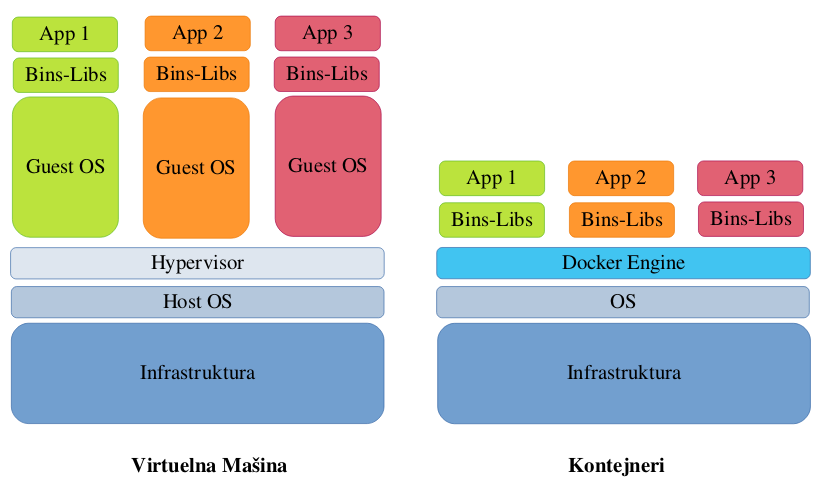
\includegraphics[width=\linewidth]{images/vm.png}
    \caption{Razlika između arhitekture Virtuelne Mašine a arhitekture kontejnera}
\end{figure}

\chapter{Teorijske osnove}
U ovom poglavlju će biti ukratko objašnjeni svi koncepti i alati koji su bili potrebni za izradu projekta o kojem ovaj rad govori. NABROJ
\section{Open source razvoj}
\section{Python, PyPI}
\section{Github}
\section{Github akcije - mozda spojiti sa prethodnim}
\section{Python paketi}

\section{Poetry}
Poetry \cite{poetry} je alat otvorenog koda (eng.\ \textit{open-source}) za kreiranje Python paketa i upravljanje paketima koje Python projekat koristi(eng.\ \textit{dependency management}). Pomaže korisnicima tako što umesto njih instalira i menja verzije  bibliotekama od kojih projekat zavisi, a koje korisnik mora pretkodno da specificira. Poetry je takođe znatno olakšao kreiranje, pakovanje i objavljivanje paketa na PyPI - repozitorijum softvera za Python programski jezik i time omogućio lakše deljenje Python projekata sa drugim korisnicima tog jezika.

Prva verzija alata objavljena je 28.02.2018. godine. Verzije programskog jezika Python koje su podržane su 2.7 i 3.4+. Ideja je da Poetry radi podjednako dobro na različitim platformama, između ostalog na Linux-u, Windows-u i OSX-u.

\subsection{Podešavanje Poetry-ja}
Za razliku od drugih Python alata za upravljanje paketima od kojih projekat zavisi, umesto pip-a - instalera za Python pakete, Poetry koristi svoj specifičan način za instalaciju. Instalator doda Poetry u korisnički direktorijum, tako da može da se koristi sa bilo kojom verzijom Python-a. Omogućena je i instalacija Poetry-ja korišćenjem pip-a, ali se ne proporučuje iz dva razloga:

\begin{enumerate}
    \item može dovesti do konflikta sa drugim sistemskim fajlovima
    \item otežava održavanje konzistentnosti pre korišćenju različitih verzija Python-a i različitih virtuelnih okruženja (eng.\ \textit{virtual environments})
\end{enumerate}

\subsection{Kreiranje Python projekta koji koristi Poetry}
Nakon isntalacije alata, moguće je kreirati projekat koji koristi Poetry za upravljanje paketima ili dodati Poetry u postojeći projekat i time kreirati virtuelno okruženje u kojem će se izvršavati naredne akcije. U oba slučaja će se kreirati \textit{pyproject.toml} datoteka koja čuva sve bitne informacije o projektu. U početku ova datoteka sadrži samo osnovne informacije o projektu:

\begin{samepage}
    \begin{verbatim}
    [tool.poetry]
    name = "poetry-demo"
    version = "0.1.0"
    description = ""
    authors = ["Name Surname <email>"]

    [tool.poetry.dependencies]
    python = "*"

    [tool.poetry.dev-dependencies]
    pytest = "^3.4"
    \end{verbatim}
\end{samepage}

Informacije o samom projektu, njegovom autoru, verziji, licenci, opisu, dokumentaciji, itd. nalaze se u prvom segmentu - \texttt{[tool.poetry]}. Informacije o paketima koje projekat koristi nalaze se u naredne dve sekcije - \texttt{[tool.poetry.dependencies]} i \texttt{[tool.poetry.dev-dependencies]}, gde se u prvoj od ove dve sekcije nalaze informacije o paketima koji se koriste u produkcionom okruženju, a u drogoj informacije o paketima koji se koriste u toku razvoja projekta. Pri instalaciji novog paketa, njegov naziv i verzija će se dopisati u jednu od ove dve sekcije, ili u obe ako je to potrebno.

Ovu datoteku je moguće ručno menjati, ali se sa njom najčešće interaguje pozivanjem poetry komandi u konzoli. Neke od tih komandi su:

\begin{itemize}
    \item \texttt{poetry add} - dodaje novi paket u \textit{pyproject.toml} datoteku
    \item \texttt{poetry remove} - briše paket iz projekta
\end{itemize}

Komande koje takođe interaguju sa \textit{pyproject.toml} datotekom, ali je ne menjaju su:

\begin{itemize}
    \item \texttt{poetry install} - instalira pakete definisane u \textit{pyproject.toml} datoteci
    \item \texttt{poetry update} - ažurira pakete u skladu sa verzijama koje pišu u \textit{pyproject.toml} datoteci
    \item \texttt{poetry lock} - zaključava pakete u prijektu
    \item \texttt{poetry check} - proverava ispravnost \textit{pyproject.toml} datoteke
\end{itemize}

Za pokretanje komandi u virtuelnom okruženju opsisanom u \textit{pyproject.toml} datoteci koristi se komanda:

\begin{itemize}
    \item \texttt{poetry run}
\end{itemize}

Za sve ostale detalje najbolje je pogledati dokumentaciju pomoću komande:

\begin{itemize}
    \item \texttt{poetry help}
\end{itemize}

\subsection{Kreiranje, pakovanje i objavljivanje Python paketa}
Da bi se Python projekat mogao objaviti, potrebno je kreirati arhivu sa svim potrebnim konfiguracijama za njega. To se postiže upotrebom komande:

\begin{itemize}
    \item \texttt{poetry build}
\end{itemize}

Nakon toga, paket je spreman za objavljivanje. U projektu se pojavi novi direktorijum sa nazivom \texttt{dist} i u njemu se nalaze dve datoteke:

\begin{enumerate}
    \item \texttt{poetry-demo-0.1.0-py2.py3-none-any.whl}
    \item \texttt{poetry-demo-0.1.0.tar.gz}
\end{enumerate}

Repozitorijum na kojem se paket objavljuje se podešava pomoću komande:

\begin{itemize}
    \item \texttt{poetry config}
\end{itemize}

Paket se objavljuje pozivanjem komande:

\begin{itemize}
    \item \texttt{poetry publish}
\end{itemize}

U tom momentu, paket postaje dostupan na izabranom repozitorijumu i svako ko ima pristup repozitorijumu može da instalira paket. Najčešće se paketi objavljuju na PyPI repozitorijumu.

\section{Bash}

\chapter{Specifikacija i implementacija projekta}
\section{pjisp-assignment-template}
\section{pjisp-template-name}
\subsection{način imenovanja repo-a}
\section{pjisp-diff}
\section{poetry-publish action}
Koristi se za publishovanje pjisp-diff i pjisp-template-name
\section{Error code u smoke-test-u - zasto je potreban?}


\chapter{Primeri korišćenja}
\chapter{Diskusija i zakljuci}
\section{Da li su github akcije spremne za produkciju?}
\chapter{Literatura}
\sloppy
\printbibliography[heading=none]

\end{document}
